\documentclass[11pt]{article}
\usepackage[notes]{la}
\lamodule{2}{2}{The Inverse of a Matrix}
\laxdoc{1.4}
\laxdoc{1.8}
\laxdoc{1.9}
\laxdoc{2.1}

\begin{document}

\section{The Inverse of a Matrix}

\begin{guide}
To solve $5x=10$ we multiply by $5^{-1}$, the number that undoes multiplication by $5$. Can we do the same for $A\bv{x}=\bv{b}$? What would a matrix $A^{-1}$ that ``undoes $A$'' have to do to the plane, which matrices have one, and how do we find it? And what has the quantity $ad-bc$ got to do with it?
\end{guide}

\textbf{By the end of this section you should be able to:}
\begin{itemize}
  \item define an invertible matrix and its inverse, and verify a proposed inverse by multiplying in \emph{both} orders;
  \item explain the inverse of a matrix as the map that undoes the original, and recognise which plane maps can be undone;
  \item use the $2\times2$ formula, and explain with a picture why $ad-bc=0$ means that no inverse exists;
  \item solve $A\bv{x}=\bv{b}$ with $A^{-1}$, and say when it is wiser not to;
  \item use $(A^{-1})^{-1}=A$, $(AB)^{-1}=B^{-1}A^{-1}$ and $(A\T)^{-1}=(A^{-1})\T$;
  \item describe elementary matrices, and explain why multiplying by one on the left performs a row operation;
  \item find $A^{-1}$ by row reducing $[A\ \ I]$, recognise a matrix with no inverse, and explain why the algorithm works;
  \item connect ``invertible'' with ``one-to-one and onto'' and with ``row equivalent to $I$''.
\end{itemize}

% ---------------------------------------------------------------------
\subsection*{Undoing a map}

For a nonzero number $a$ the number $a^{-1}$ satisfies $a^{-1}a=1=aa^{-1}$. Multiplication by $a^{-1}$ undoes multiplication by $a$. In Section~1.9 (Pause and think~\ref{1.9-think:undo}) we met the same idea for plane maps: the rotation by $\theta$ is undone by the rotation by $-\theta$, and a shear is undone by the shear in the opposite direction. The identity matrix $I$ is the map that does nothing, so ``undo'' means ``compose to get $I$''.

\begin{defn}{Invertible matrix}{inverse}
An $n\times n$ matrix $A$ is \emph{invertible} if there is an $n\times n$ matrix $C$ with
\[
CA=I\qquad\text{and}\qquad AC=I .
\]
Such a $C$ is called an \emph{inverse} of $A$. A matrix that is not invertible is sometimes called \emph{singular}.
\end{defn}

The two equations say two things. $CA=I$ means that $C$ undoes $A$: $C(A\bv{x})=\bv{x}$. $AC=I$ means that $A$ undoes $C$: $A(C\bv{y})=\bv{y}$. For numbers the two conditions coincide because $ab=ba$; for matrices we know from Section~2.1 that order can matter, so the definition asks for both.

\begin{thm}{The inverse is unique}{unique}
If $A$ is invertible, then it has only one inverse. It is denoted $A^{-1}$, so that $A^{-1}A=I=AA^{-1}$.
\end{thm}

\begin{proof}
Suppose $B$ and $C$ are both inverses of $A$. Then, using associativity (Theorem~\ref{2.1-thm:mulprops}),
\[
B=BI=B(AC)=(BA)C=IC=C.
\]
\end{proof}

\begin{warn}[Only square matrices and no division]
Only \emph{square} matrices are asked to have inverses here, and $A^{-1}$ is \emph{not} a fraction: never write $\tfrac1A$ or $\bv{b}/A$. Because $AB\neq BA$ in general, ``dividing by $A$'' would not even say on which side. We write $A^{-1}\bv{b}$ and $BA^{-1}$, and they are different things.
\end{warn}

\begin{exmp}{Checking a proposed inverse}{check}
Let $A=\begin{bmatrix}2&5\\-3&-7\end{bmatrix}$ and $C=\begin{bmatrix}-7&-5\\3&2\end{bmatrix}$. Then
\[
AC=\begin{bmatrix}2\cdot(-7)+5\cdot3&2\cdot(-5)+5\cdot2\\-3\cdot(-7)-7\cdot3&-3\cdot(-5)-7\cdot2\end{bmatrix}=\begin{bmatrix}1&0\\0&1\end{bmatrix},\qquad
CA=\begin{bmatrix}-14+15&-35+35\\6-6&15-14\end{bmatrix}=\begin{bmatrix}1&0\\0&1\end{bmatrix}.
\]
Both products are $I$, so $A$ is invertible and $A^{-1}=C$.
\end{exmp}

\begin{exmp}{Inverses we already know}{known}
\textbf{(a) Rotation.} By Section~1.9, $R_\varphi R_\theta=R_{\varphi+\theta}$, so $R_{-\theta}R_\theta=R_0=I=R_\theta R_{-\theta}$. Hence $R_\theta^{-1}=R_{-\theta}=\begin{bmatrix}\cos\theta&\sin\theta\\-\sin\theta&\cos\theta\end{bmatrix}$, which is also the transpose $R_\theta\T$ (Definition~\ref{2.1-def:transpose}).

\textbf{(b) Shear.} For $S=\begin{bmatrix}1&1\\0&1\end{bmatrix}$, Example~\ref{2.1-ex:shearpowers} gave $S^k=\begin{bmatrix}1&k\\0&1\end{bmatrix}$. The choice $k=-1$ suggests $S^{-1}=\begin{bmatrix}1&-1\\0&1\end{bmatrix}$, and indeed
\[
\begin{bmatrix}1&-1\\0&1\end{bmatrix}\begin{bmatrix}1&1\\0&1\end{bmatrix}=\begin{bmatrix}1&0\\0&1\end{bmatrix}=\begin{bmatrix}1&1\\0&1\end{bmatrix}\begin{bmatrix}1&-1\\0&1\end{bmatrix}.
\]

\textbf{(c) Reflection.} For $F=\begin{bmatrix}1&0\\0&-1\end{bmatrix}$ we have $F^2=I$ (Knowledge Check~\ref{1.9-kc:reflect}), so $F^{-1}=F$: a reflection undoes itself.
\end{exmp}

Some matrices cannot be undone, and there is a quick test that catches many of them.

\begin{thm}{A nonzero vector sent to zero}{noninv}
If $A\bv{x}=\bv{0}$ for some $\bv{x}\neq\bv{0}$, then $A$ is not invertible.
\end{thm}

\begin{proof}
If $C$ were an inverse, then $\bv{x}=I\bv{x}=(CA)\bv{x}=C(A\bv{x})=C\bv{0}=\bv{0}$, contradicting $\bv{x}\neq\bv{0}$.
\end{proof}

For example the projection $P=\begin{bmatrix}1&0\\0&0\end{bmatrix}$ of Section~1.8 has $P\bv{e}_2=\bv{0}$, so it is not invertible: all the points of a vertical line are sent to one point, and no map can tell which one we started from. The matrix of Example~\ref{2.1-ex:zerodiv} sends $(1,-1)$ to $\bv{0}$ and is not invertible either.

\begin{center}
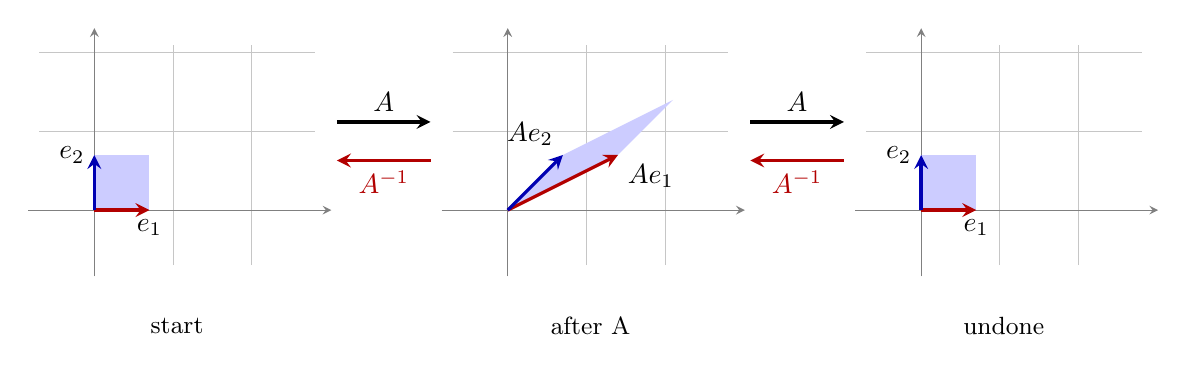
\begin{tikzpicture}[x=0.7cm,y=0.7cm,>=stealth]
  \draw[gray!45] (-1,-1) grid (4,3);
  \draw[->,gray] (-1.2,0)--(4.3,0); \draw[->,gray] (0,-1.2)--(0,3.3);
  \fill[blue!20] (0,0) rectangle (1,1);
  \draw[->,very thick,red!70!black] (0,0)--(1,0);
  \draw[->,very thick,blue!70!black] (0,0)--(0,1);
  \node[below] at (1,0) {$e_1$};
  \node[left] at (0,1) {$e_2$};
  \node at (1.5,-2.1) {\small start};
  \draw[->,very thick] (4.4,1.6)--(6.1,1.6) node[midway,above] {$A$};
  \draw[->,very thick,red!70!black] (6.1,0.9)--(4.4,0.9) node[midway,below] {$A^{-1}$};
  \begin{scope}[shift={(7.5,0)}]
    \draw[gray!45] (-1,-1) grid (4,3);
    \draw[->,gray] (-1.2,0)--(4.3,0); \draw[->,gray] (0,-1.2)--(0,3.3);
    \fill[blue!20] (0,0)--(2,1)--(3,2)--(1,1)--cycle;
    \draw[->,very thick,red!70!black] (0,0)--(2,1);
    \draw[->,very thick,blue!70!black] (0,0)--(1,1);
    \node[below right] at (2,1) {$Ae_1$};
    \node[above left] at (1,1) {$Ae_2$};
    \node at (1.5,-2.1) {\small after A};
    \draw[->,very thick] (4.4,1.6)--(6.1,1.6) node[midway,above] {$A$};
    \draw[->,very thick,red!70!black] (6.1,0.9)--(4.4,0.9) node[midway,below] {$A^{-1}$};
  \end{scope}
  \begin{scope}[shift={(15,0)}]
    \draw[gray!45] (-1,-1) grid (4,3);
    \draw[->,gray] (-1.2,0)--(4.3,0); \draw[->,gray] (0,-1.2)--(0,3.3);
    \fill[blue!20] (0,0) rectangle (1,1);
    \draw[->,very thick,red!70!black] (0,0)--(1,0);
    \draw[->,very thick,blue!70!black] (0,0)--(0,1);
    \node[below] at (1,0) {$e_1$};
    \node[left] at (0,1) {$e_2$};
    \node at (1.5,-2.1) {\small undone};
  \end{scope}
\end{tikzpicture}
\end{center}

\textbf{Figure.} The matrix $A=\begin{bmatrix}2&1\\1&1\end{bmatrix}$ sends $\bv{e}_1$ to $(2,1)$ and $\bv{e}_2$ to $(1,1)$ and the unit square to the parallelogram with corners $(0,0),(2,1),(3,2),(1,1)$. The matrix $A^{-1}=\begin{bmatrix}1&-1\\-1&2\end{bmatrix}$ sends $(2,1)$ back to $\bv{e}_1$ and $(1,1)$ back to $\bv{e}_2$, so it carries the parallelogram back to the square: first $A$, then $A^{-1}$, changes nothing.

\begin{kc}{Guess and check}{guess}
Write down the inverse of each matrix by thinking about what it does to the plane, then check your answer by multiplying. (a)~$\begin{bmatrix}3&0\\0&-2\end{bmatrix}$; \ (b)~the rotation by $90^\circ$; \ (c)~$\begin{bmatrix}0&1\\1&0\end{bmatrix}$; \ (d)~$\begin{bmatrix}1&3\\0&1\end{bmatrix}$.
\end{kc}

\begin{kc}{Verify}{verify}
Is $C=\begin{bmatrix}1&-1\\-1&2\end{bmatrix}$ the inverse of $A=\begin{bmatrix}2&1\\1&1\end{bmatrix}$? Is $D=\begin{bmatrix}1&1\\1&2\end{bmatrix}$? Multiply in both orders for the matrix that works.
\end{kc}

\begin{think}{Why two equations?}{twoeq}
(a)~In Definition~\ref{def:inverse} the matrix $C$ must satisfy $CA=I$ \emph{and} $AC=I$. Explain in terms of maps what each says. (b)~In the proof of Theorem~\ref{thm:unique} which of the two equations was used for $B$ and which for $C$?
\end{think}

\begin{think}{Which maps can be undone?}{whichundo}
Look back at the plane maps of Section~1.9: rotations, reflections, shears, stretches and the projection. Which can be undone? To undo a map $T$ we must be able to find, for every output $\bv{y}$, the input $\bv{x}$ that produced it, and the input must be the only one. Which two properties of Section~1.9 does that require?
\end{think}

% ---------------------------------------------------------------------
\subsection*{The $2\times2$ case and the number $ad-bc$}

For $2\times2$ matrices there is a formula.

\begin{thm}{The inverse of a $2\times2$ matrix}{twobytwo}
Let $A=\begin{bmatrix}a&b\\c&d\end{bmatrix}$ and put $\Delta=ad-bc$.
\begin{enumerate}[label=(\alph*),itemsep=1pt]
  \item If $\Delta\neq0$, then $A$ is invertible and
  \[
  A^{-1}=\frac1{ad-bc}\begin{bmatrix}d&-b\\-c&a\end{bmatrix}.
  \]
  \item If $\Delta=0$, then $A$ is not invertible.
\end{enumerate}
\end{thm}

\begin{proof}
(a)~Multiply: $\begin{bmatrix}a&b\\c&d\end{bmatrix}\begin{bmatrix}d&-b\\-c&a\end{bmatrix}=\begin{bmatrix}ad-bc&-ab+ba\\cd-dc&-cb+da\end{bmatrix}=\begin{bmatrix}\Delta&0\\0&\Delta\end{bmatrix}$, and the product in the other order is the same. Dividing by $\Delta$ gives $I$ in both orders.

(b)~Suppose $\Delta=0$. The vector $(d,-c)$ satisfies $A(d,-c)=(ad-bc,\ cd-dc)=(0,0)$. If $(d,-c)\neq\bv{0}$, Theorem~\ref{thm:noninv} shows that $A$ is not invertible. Otherwise $c=d=0$, and then $A(b,-a)=(ab-ba,\ cb-da)=\bv{0}$; if $(b,-a)\neq\bv{0}$ we are done in the same way. If also $a=b=0$, then $A=\mathbf{0}$ and $A$ has no inverse because $\mathbf{0}C=\mathbf{0}\neq I$.
\end{proof}

The number $ad-bc$ is called the \emph{determinant} of $A$. It is not an arbitrary condition. In Section~1.9 (Pause and think~\ref{1.9-think:area}) you computed that the image of the unit square is the parallelogram on the two columns, with area $|ad-bc|$.

\begin{center}
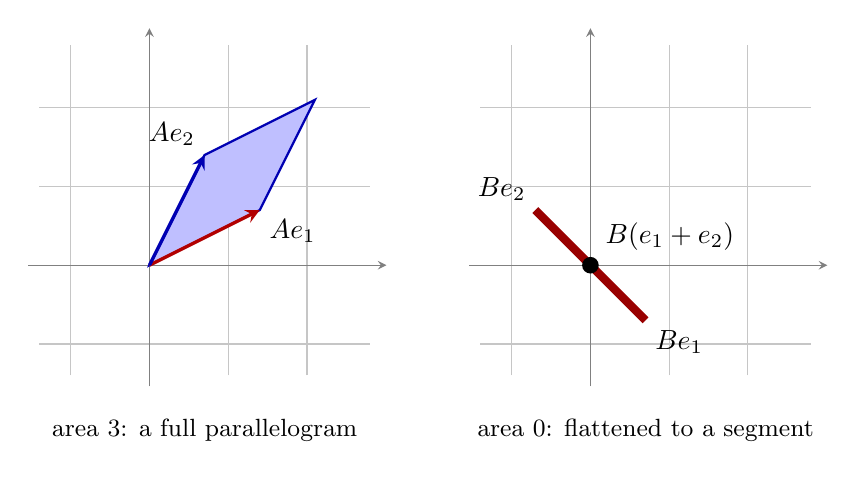
\begin{tikzpicture}[x=0.7cm,y=0.7cm,>=stealth]
  \draw[gray!45] (-2,-2) grid (4,4);
  \draw[->,gray] (-2.2,0)--(4.3,0); \draw[->,gray] (0,-2.2)--(0,4.3);
  \fill[blue!25] (0,0)--(2,1)--(3,3)--(1,2)--cycle;
  \draw[thick,blue!70!black] (0,0)--(2,1)--(3,3)--(1,2)--cycle;
  \draw[->,very thick,red!70!black] (0,0)--(2,1);
  \draw[->,very thick,blue!70!black] (0,0)--(1,2);
  \node[below right] at (2,1) {$Ae_1$};
  \node[above left] at (1,2) {$Ae_2$};
  \node at (1,-3.0) {\small area 3: a full parallelogram};
  \begin{scope}[shift={(8,0)}]
    \draw[gray!45] (-2,-2) grid (4,4);
    \draw[->,gray] (-2.2,0)--(4.3,0); \draw[->,gray] (0,-2.2)--(0,4.3);
    \draw[line width=3pt,red!60!black] (-1,1)--(1,-1);
    \fill (0,0) circle (3pt);
    \node[below right] at (1,-1) {$Be_1$};
    \node[above left] at (-1,1) {$Be_2$};
    \node[above right] at (0.1,0.1) {$B(e_1+e_2)$};
    \node at (1,-3.0) {\small area 0: flattened to a segment};
  \end{scope}
\end{tikzpicture}
\end{center}

\textbf{Figure.} Left: $A=\begin{bmatrix}2&1\\1&2\end{bmatrix}$ has $ad-bc=3$, the area of the image of the unit square. Right: $B=\begin{bmatrix}1&-1\\-1&1\end{bmatrix}$ has $ad-bc=0$. The square is flattened onto a segment: $B\bv{e}_1=(1,-1)$, $B\bv{e}_2=(-1,1)$ and $B(\bv{e}_1+\bv{e}_2)=\bv{0}$. Whole lines (those parallel to $(1,1)$) are crushed to single points, so nothing can restore the original positions.

So $ad-bc=0$ means that the two columns lie on one line, the map flattens the plane, some nonzero vector is sent to $\bv{0}$, and the matrix is not invertible. In Section~1.9 you saw that a flattening map is neither one-to-one nor onto.

\begin{exmp}{Using the formula}{formula}
For $A=\begin{bmatrix}3&4\\5&6\end{bmatrix}$ we get $ad-bc=18-20=-2\neq0$, so
\[
A^{-1}=\frac1{-2}\begin{bmatrix}6&-4\\-5&3\end{bmatrix}=\begin{bmatrix}-3&2\\\tfrac52&-\tfrac32\end{bmatrix}.
\]
Check: $AA^{-1}=\begin{bmatrix}3(-3)+4\cdot\tfrac52&3\cdot2+4(-\tfrac32)\\5(-3)+6\cdot\tfrac52&5\cdot2+6(-\tfrac32)\end{bmatrix}=\begin{bmatrix}-9+10&6-6\\-15+15&10-9\end{bmatrix}=I$. \ $\checkmark$ The determinant is negative, so this map reverses orientation (compare the reflection in Section~1.9).
\end{exmp}

\begin{exmp}{A parameter}{param}
For which $h$ is $A=\begin{bmatrix}1&h\\2&4\end{bmatrix}$ invertible? Find $A^{-1}$ when it exists.

\textbf{Solution.} $ad-bc=4-2h$, which is $0$ exactly when $h=2$. For $h=2$ the columns $(1,2)$ and $(2,4)$ are multiples of each other, the plane is flattened onto a line, and $A$ is not invertible. For every $h\neq2$,
\[
A^{-1}=\frac1{4-2h}\begin{bmatrix}4&-h\\-2&1\end{bmatrix}.
\]
For instance $h=0$ gives $A^{-1}=\tfrac14\begin{bmatrix}4&0\\-2&1\end{bmatrix}=\begin{bmatrix}1&0\\-\tfrac12&\tfrac14\end{bmatrix}$, and one checks $\begin{bmatrix}1&0\\2&4\end{bmatrix}\begin{bmatrix}1&0\\-\tfrac12&\tfrac14\end{bmatrix}=\begin{bmatrix}1&0\\2-2&1\end{bmatrix}=I$.
\end{exmp}

\subsection*{Solving $A\bv{x}=\bv{b}$ with the inverse}

\begin{thm}{Solving with the inverse}{solve}
If $A$ is an invertible $n\times n$ matrix, then for every $\bv{b}$ in $\R^n$ the equation $A\bv{x}=\bv{b}$ has the \emph{unique} solution $\bv{x}=A^{-1}\bv{b}$.
\end{thm}

\begin{proof}
Existence: $A(A^{-1}\bv{b})=(AA^{-1})\bv{b}=I\bv{b}=\bv{b}$. Uniqueness: if $A\bv{x}=\bv{b}$, multiply both sides on the \emph{left} by $A^{-1}$: $\bv{x}=A^{-1}A\bv{x}=A^{-1}\bv{b}$.
\end{proof}

\begin{exmp}{Solving a system with the inverse}{solvesys}
Solve $3x_1+4x_2=3$, \ $5x_1+6x_2=7$. This is $A\bv{x}=\bv{b}$ with the matrix $A$ of Example~\ref{ex:formula} and $\bv{b}=(3,7)$. Then
\[
\bv{x}=A^{-1}\bv{b}=\begin{bmatrix}-3&2\\\tfrac52&-\tfrac32\end{bmatrix}\begin{bmatrix}3\\7\end{bmatrix}=\begin{bmatrix}-9+14\\\tfrac{15}2-\tfrac{21}2\end{bmatrix}=\begin{bmatrix}5\\-3\end{bmatrix}.
\]
Check: $3\cdot5+4(-3)=3$ and $5\cdot5+6(-3)=7$. \ $\checkmark$ The same $A^{-1}$ solves the system for every other right-hand side with two multiplications by it.
\end{exmp}

\begin{warn}[Inverse or row reduction]
Finding $A^{-1}$ takes about as much work as solving $n$ systems with the same matrix. To solve \emph{one} system, row reduce $[A\ \ \bv{b}]$ as in Chapter~1; computing the inverse first is wasteful. The inverse is valuable for \emph{understanding} (it is the undoing map and it satisfies simple algebra) and for many right-hand sides. Never compute $A^{-1}$ just to solve a single system.
\end{warn}

\begin{kc}{The formula and a system}{formulakc}
Let $A=\begin{bmatrix}7&3\\5&2\end{bmatrix}$. (a)~Find $A^{-1}$ with the formula. (b)~Solve $A\bv{x}=(1,2)$. (c)~Is $\begin{bmatrix}2&4\\3&6\end{bmatrix}$ invertible?
\end{kc}

\begin{think}{Why $ad-bc$?}{whydet}
(a)~Without the formula: if the two columns of $A=\begin{bmatrix}a&b\\c&d\end{bmatrix}$ are multiples of each other, explain geometrically (with the unit square) why $A$ cannot be undone. (b)~The matrix $\begin{bmatrix}0&1\\1&0\end{bmatrix}$ has $ad-bc=-1$ and the rotation has $+1$; both are invertible. What does a negative value of $ad-bc$ tell you about the picture? (c)~The map with matrix $\begin{bmatrix}2&0\\0&2\end{bmatrix}$ has $ad-bc=4$. Its inverse has $ad-bc$ equal to what? Why is that reasonable?
\end{think}

\begin{think}{Inverse or row reduction?}{manyb}
Suppose you must solve $A\bv{x}=\bv{b}_k$ for $1000$ different vectors $\bv{b}_k$, with the same invertible $A$. (a)~Why does this favour computing $A^{-1}$ once? (b)~Using the counts from Section~2.1 (Pause and think~\ref{2.1-think:assoccost}), is the matrix--vector product cheap compared with the cost of $A^{-1}$ itself?
\end{think}

% ---------------------------------------------------------------------
\subsection*{Inverses of products and transposes}

\begin{thm}{Algebra of inverses}{invprops}
Let $A$ and $B$ be invertible $n\times n$ matrices.
\begin{enumerate}[label=(\alph*),itemsep=1pt]
  \item $A^{-1}$ is invertible and $(A^{-1})^{-1}=A$.
  \item $AB$ is invertible and $(AB)^{-1}=B^{-1}A^{-1}$ \quad (the order is \textbf{reversed}).
  \item $A\T$ is invertible and $(A\T)^{-1}=(A^{-1})\T$.
\end{enumerate}
\end{thm}

\begin{proof}
(a)~$A^{-1}A=I=AA^{-1}$ says that $A$ is an inverse of $A^{-1}$.

(b)~Check both products with associativity: $(AB)(B^{-1}A^{-1})=A(BB^{-1})A^{-1}=AIA^{-1}=AA^{-1}=I$, and $(B^{-1}A^{-1})(AB)=B^{-1}(A^{-1}A)B=B^{-1}B=I$.

(c)~By Theorem~\ref{2.1-thm:transprops}(d), $A\T(A^{-1})\T=(A^{-1}A)\T=I\T=I$ and $(A^{-1})\T A\T=(AA^{-1})\T=I$.
\end{proof}

Part (b) has a plain meaning. If we do $B$ and then $A$, we undo it by undoing $A$ first and then $B$.

\begin{center}
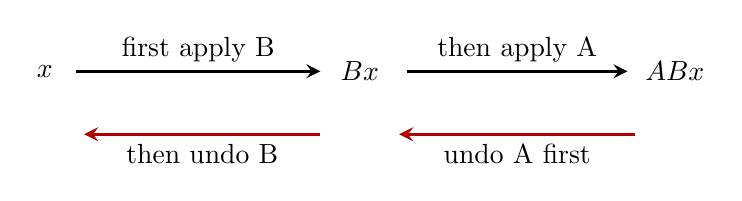
\begin{tikzpicture}[>=stealth]
  \node (a) at (0,1.2) {$x$};
  \node (b) at (4,1.2) {$Bx$};
  \node (c) at (8,1.2) {$ABx$};
  \draw[->,very thick] (0.4,1.2)--(3.5,1.2); \node[above] at (1.95,1.2) {first apply B};
  \draw[->,very thick] (4.6,1.2)--(7.4,1.2); \node[above] at (6,1.2) {then apply A};
  \draw[->,very thick,red!70!black] (7.5,0.4)--(4.5,0.4); \node[below] at (6,0.4) {undo A first};
  \draw[->,very thick,red!70!black] (3.5,0.4)--(0.5,0.4); \node[below] at (2,0.4) {then undo B};
\end{tikzpicture}
\end{center}

\textbf{Figure.} The inverse of ``$B$ then $A$'' takes the steps back in the opposite order: $(AB)^{-1}=B^{-1}A^{-1}$.

\begin{exmp}{The inverse of a product}{prodinv}
Let $A=\begin{bmatrix}1&1\\0&1\end{bmatrix}$ (a shear) and $B=\begin{bmatrix}2&0\\0&1\end{bmatrix}$ (a stretch). Then $A^{-1}=\begin{bmatrix}1&-1\\0&1\end{bmatrix}$ and $B^{-1}=\begin{bmatrix}\tfrac12&0\\0&1\end{bmatrix}$, and $AB=\begin{bmatrix}2&1\\0&1\end{bmatrix}$ has $ad-bc=2$, so by the formula
\[
(AB)^{-1}=\frac12\begin{bmatrix}1&-1\\0&2\end{bmatrix}=\begin{bmatrix}\tfrac12&-\tfrac12\\0&1\end{bmatrix}.
\]
Compare with the product of the inverses in the reverse order:
\[
B^{-1}A^{-1}=\begin{bmatrix}\tfrac12&0\\0&1\end{bmatrix}\begin{bmatrix}1&-1\\0&1\end{bmatrix}=\begin{bmatrix}\tfrac12&-\tfrac12\\0&1\end{bmatrix}=(AB)^{-1}.
\]
In the \emph{same} order we would get $A^{-1}B^{-1}=\begin{bmatrix}\tfrac12&-1\\0&1\end{bmatrix}$, which is not the inverse.
\end{exmp}

\begin{kc}{Invert a product}{prodinvkc}
Let $A=\begin{bmatrix}2&0\\0&3\end{bmatrix}$ and $B=\begin{bmatrix}1&2\\0&1\end{bmatrix}$. Find $A^{-1}$, $B^{-1}$ and $(AB)^{-1}$, using $(AB)^{-1}=B^{-1}A^{-1}$, and check by multiplying $AB$ by your answer.
\end{kc}

\begin{think}{Sums and inverses}{sums}
(a)~Find two invertible $2\times2$ matrices whose sum is not invertible. (b)~Is $(A+B)^{-1}=A^{-1}+B^{-1}$? Test $A=B=I$. (c)~Show that $(A^k)^{-1}=(A^{-1})^k$ for $k=2$ and $k=3$. What does this say about the inverse of ``apply $A$ three times''?
\end{think}

% ---------------------------------------------------------------------
\subsection*{Elementary matrices}

Row operations are the engine of Chapter~1. We now see that each one is a matrix multiplication.

\begin{defn}{Elementary matrix}{elementary}
An \emph{elementary matrix} is a matrix obtained from the identity matrix by \emph{one} elementary row operation: a replacement $R_i+cR_j\to R_i$, an interchange $R_i\leftrightarrow R_j$, or a scaling $cR_i\to R_i$ with $c\neq0$.
\end{defn}

\begin{exmp}{Three elementary matrices acting on a matrix}{elem}
Let $A=\begin{bmatrix}1&2&3\\4&5&6\\7&8&10\end{bmatrix}$. Starting from $I_3$:
\begin{align*}
E_1&=\begin{bmatrix}1&0&0\\-4&1&0\\0&0&1\end{bmatrix}\quad(R_2-4R_1\to R_2),&
E_2&=\begin{bmatrix}0&0&1\\0&1&0\\1&0&0\end{bmatrix}\quad(R_1\leftrightarrow R_3),&
E_3&=\begin{bmatrix}1&0&0\\0&1&0\\0&0&5\end{bmatrix}\quad(5R_3\to R_3).
\end{align*}
Now multiply, on the \emph{left}:
\[
E_1A=\begin{bmatrix}1&2&3\\0&-3&-6\\7&8&10\end{bmatrix},\qquad
E_2A=\begin{bmatrix}7&8&10\\4&5&6\\1&2&3\end{bmatrix},\qquad
E_3A=\begin{bmatrix}1&2&3\\4&5&6\\35&40&50\end{bmatrix}.
\]
Each product is $A$ with the same row operation applied: $E_1A$ replaced row $2$ by row $2$ minus $4$ times row $1$, $E_2A$ swapped rows $1$ and $3$, $E_3A$ multiplied row $3$ by $5$.
\end{exmp}

\begin{thm}{Elementary matrices}{elementary}
Let $E$ be the $m\times m$ elementary matrix of a row operation.
\begin{enumerate}[label=(\alph*),itemsep=1pt]
  \item For every $m\times p$ matrix $A$, the product $EA$ is the matrix obtained from $A$ by performing that row operation.
  \item $E$ is invertible, and $E^{-1}$ is the elementary matrix of the \emph{reverse} row operation (of the same kind).
\end{enumerate}
\end{thm}

\begin{proof}
(a)~By Theorem~\ref{2.1-thm:rowview}, row $i$ of $EA$ is (row $i$ of $E$)$\,A$, a combination of the rows of $A$ with weights from row $i$ of $E$. Every row of $E$ equals the corresponding row of $I$, except the one row that the operation changed. A row of $I$ (a $1$ in position $i$) gives back row $i$ of $A$, so the unchanged rows of $EA$ are those of $A$. For the changed row, say $R_i+cR_j\to R_i$, row $i$ of $E$ is $\bv{e}_i\T+c\,\bv{e}_j\T$ and row $i$ of $EA$ is (row $i$ of $A$)$+c\,$(row $j$ of $A$). The interchange and the scaling are the same argument.

(b)~Let $E'$ be the elementary matrix of the reverse operation ($R_i-cR_j\to R_i$, or the same interchange, or $\tfrac1cR_i\to R_i$). By part (a), $E'E$ is the matrix obtained by performing the operation and then its reverse on $I$, which is $I$. In the same way $EE'=I$.
\end{proof}

\begin{center}
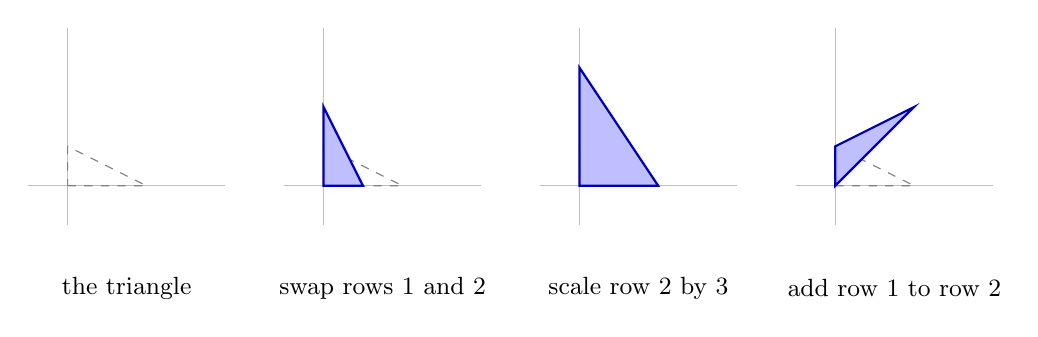
\begin{tikzpicture}[x=0.5cm,y=0.5cm,>=stealth]
  \foreach \cx in {0,6.5,13,19.5}{
    \begin{scope}[shift={(\cx,0)}]
      \draw[gray!50] (-1,0)--(4,0); \draw[gray!50] (0,-1)--(0,4);
      \draw[dashed,gray] (0,0)--(2,0)--(0,1)--cycle;
    \end{scope}}
  \begin{scope}[shift={(0,0)}]
    \node at (1.5,-2.6) {\small the triangle};
  \end{scope}
  \begin{scope}[shift={(6.5,0)}]
    \draw[thick,blue!70!black,fill=blue!25] (0,0)--(0,2)--(1,0)--cycle;
    \node at (1.5,-2.6) {\small swap rows 1 and 2};
  \end{scope}
  \begin{scope}[shift={(13,0)}]
    \draw[thick,blue!70!black,fill=blue!25] (0,0)--(2,0)--(0,3)--cycle;
    \node at (1.5,-2.6) {\small scale row 2 by 3};
  \end{scope}
  \begin{scope}[shift={(19.5,0)}]
    \draw[thick,blue!70!black,fill=blue!25] (0,0)--(2,2)--(0,1)--cycle;
    \node at (1.5,-2.6) {\small add row 1 to row 2};
  \end{scope}
\end{tikzpicture}
\end{center}

\textbf{Figure.} What the $2\times2$ elementary matrices $\begin{bmatrix}0&1\\1&0\end{bmatrix}$, $\begin{bmatrix}1&0\\0&3\end{bmatrix}$ and $\begin{bmatrix}1&0\\1&1\end{bmatrix}$ do to the triangle with corners $(0,0),(2,0),(0,1)$ (dashed): the interchange is the reflection in the line $x_2=x_1$, the scaling stretches vertically by $3$, and the replacement is a shear. Each can be undone by the elementary matrix of the reverse operation: swap again, scale by $\tfrac13$, subtract row $1$ from row $2$.

\begin{kc}{Elementary matrices}{elemkc}
For $3\times3$ matrices write (a)~the elementary matrix $E$ for $R_3+5R_1\to R_3$ and its inverse; (b)~the elementary matrix for $R_2\leftrightarrow R_3$ and its inverse; (c)~the elementary matrix for $\tfrac12R_2\to R_2$ and its inverse. Which of the three is its own inverse?
\end{kc}

\begin{think}{Elementary matrices as plane maps}{elemmaps}
(a)~Which of the three pictures above flattens the triangle? Why could none of them? (b)~Every elementary matrix is invertible. How is this related to the fact that every row operation can be reversed (Section~1.1)? (c)~Why is it essential that the scaling factor is $c\neq0$?
\end{think}

% ---------------------------------------------------------------------
\subsection*{An algorithm for the inverse}

Suppose row operations take $A$ to $I$. Then there are elementary matrices with $E_p\cdots E_2E_1A=I$, so the product $C=E_p\cdots E_1$ satisfies $CA=I$. But the same product is $C=E_p\cdots E_1I$: the operations that reduce $A$ to $I$ turn $I$ into $C$. This is the algorithm; the theorem says that it works and that it is the only way to find an inverse.

\begin{thm}{Invertible means row equivalent to $I$}{algorithm}
An $n\times n$ matrix $A$ is invertible if and only if $A$ is row equivalent to $I_n$. In that case, any sequence of row operations that reduces $A$ to $I_n$ also transforms $I_n$ into $A^{-1}$.
\end{thm}

\begin{proof}
($\Leftarrow$)~Let $E_p\cdots E_1A=I$ and $C=E_p\cdots E_1$, so $CA=I$. Each $E_k$ is invertible (Theorem~\ref{thm:elementary}(b)), so $C$ is invertible with $C^{-1}=E_1^{-1}\cdots E_p^{-1}$ by repeated use of Theorem~\ref{thm:invprops}(b). Then $A=C^{-1}(CA)=C^{-1}$, hence $AC=C^{-1}C=I$. So $C=A^{-1}$, and $C=C\,I$ is exactly what the row operations make of $I$.

($\Rightarrow$)~Let $A$ be invertible. For every $\bv{b}$ the equation $A\bv{x}=\bv{b}$ has the solution $A^{-1}\bv{b}$ (Theorem~\ref{thm:solve}), so $A$ has a pivot in every row (Theorem~\ref{1.4-thm:existence}). A square $n\times n$ matrix with $n$ pivots has one in every column as well, so its reduced echelon form is $I_n$.
\end{proof}

\begin{proc}{Finding $A^{-1}$}{inverse}
\begin{enumerate}
  \item Form the $n\times2n$ matrix $[A\ \ I]$.
  \item Row reduce it. If the left half becomes $I$, the right half is $A^{-1}$: $[A\ \ I]\to[I\ \ A^{-1}]$.
  \item If the left half acquires a row of zeros (so $A$ is not row equivalent to $I$), then $A$ is not invertible.
  \item Check: multiply $A$ by the matrix you found.
\end{enumerate}
\end{proc}

\begin{exmp}{Finding an inverse}{algo}
Find the inverse of $A=\begin{bmatrix}1&2&0\\0&1&3\\1&3&4\end{bmatrix}$.

\textbf{Solution.}
\begin{align*}
\begin{amat}{ccc|ccc}1&2&0&1&0&0\\0&1&3&0&1&0\\1&3&4&0&0&1\end{amat}
&\rops{R_3-R_1}
\begin{amat}{ccc|ccc}1&2&0&1&0&0\\0&1&3&0&1&0\\0&1&4&-1&0&1\end{amat}
\rops{R_3-R_2}
\begin{amat}{ccc|ccc}1&2&0&1&0&0\\0&1&3&0&1&0\\0&0&1&-1&-1&1\end{amat}\\[4pt]
&\rops{R_2-3R_3}
\begin{amat}{ccc|ccc}1&2&0&1&0&0\\0&1&0&3&4&-3\\0&0&1&-1&-1&1\end{amat}
\rops{R_1-2R_2}
\begin{amat}{ccc|ccc}1&0&0&-5&-8&6\\0&1&0&3&4&-3\\0&0&1&-1&-1&1\end{amat}.
\end{align*}
The left half is $I$, so
\[
A^{-1}=\begin{bmatrix}-5&-8&6\\3&4&-3\\-1&-1&1\end{bmatrix}.
\]
Check, first row of $AA^{-1}$: $1(-5)+2(3)+0=1$, \ $1(-8)+2(4)+0=0$, \ $1(6)+2(-3)+0=0$; third row: $-5+9-4=0$, \ $-8+12-4=0$, \ $6-9+4=1$. (The full product is $I$.) \ $\checkmark$
\end{exmp}

\begin{exmp}{A matrix with no inverse}{singular}
Try $A=\begin{bmatrix}1&2&3\\2&5&7\\3&7&10\end{bmatrix}$.
\begin{align*}
\begin{amat}{ccc|ccc}1&2&3&1&0&0\\2&5&7&0&1&0\\3&7&10&0&0&1\end{amat}
&\rops{R_2-2R_1,\ R_3-3R_1}
\begin{amat}{ccc|ccc}1&2&3&1&0&0\\0&1&1&-2&1&0\\0&1&1&-3&0&1\end{amat}
\rops{R_3-R_2}
\begin{amat}{ccc|ccc}1&2&3&1&0&0\\0&1&1&-2&1&0\\0&0&0&-1&-1&1\end{amat}.
\end{align*}
The left half has a row of zeros: $A$ has only two pivots, is not row equivalent to $I_3$, and is not invertible (Theorem~\ref{thm:algorithm}). Indeed the third row of $A$ is the sum of the first two, so the third equation of any system $A\bv{x}=\bv{b}$ is redundant or contradictory, and $A\bv{x}=\bv{b}$ has no solution for most $\bv{b}$. The last row of the right half, $\begin{bmatrix}-1&-1&1\end{bmatrix}$, records the dependence: $-R_1-R_2+R_3=\mathbf{0}$.
\end{exmp}

\begin{exmp}{Only one column of the inverse}{onecol}
The columns of $A^{-1}$ are the solutions of $A\bv{x}=\bv{e}_j$: the $j$th column of $AA^{-1}=I$ is $A(\text{column }j\text{ of }A^{-1})=\bv{e}_j$. So to find just the second column of the inverse of Example~\ref{ex:algo}, row reduce $[A\ \ \bv{e}_2]$:
\begin{align*}
\begin{amat}{ccc|c}1&2&0&0\\0&1&3&1\\1&3&4&0\end{amat}
&\rops{R_3-R_1}
\begin{amat}{ccc|c}1&2&0&0\\0&1&3&1\\0&1&4&0\end{amat}
\rops{R_3-R_2}
\begin{amat}{ccc|c}1&2&0&0\\0&1&3&1\\0&0&1&-1\end{amat}\\[4pt]
&\rops{R_2-3R_3}
\begin{amat}{ccc|c}1&2&0&0\\0&1&0&4\\0&0&1&-1\end{amat}
\rops{R_1-2R_2}
\begin{amat}{ccc|c}1&0&0&-8\\0&1&0&4\\0&0&1&-1\end{amat}.
\end{align*}
The solution $(-8,4,-1)$ is the second column of $A^{-1}$ found before. The algorithm is nothing but $n$ systems $A\bv{x}=\bv{e}_j$ solved at the same time with the same row operations.
\end{exmp}

\begin{exmp}{Undoing a map given by a formula}{mapinv}
Let $T(x_1,x_2)=(2x_1+3x_2,\ x_1+2x_2)$. Its standard matrix is $A=\begin{bmatrix}2&3\\1&2\end{bmatrix}$ with $ad-bc=4-3=1$, so $A^{-1}=\begin{bmatrix}2&-3\\-1&2\end{bmatrix}$ and the map that undoes $T$ is
\[
T^{-1}(y_1,y_2)=(2y_1-3y_2,\ -y_1+2y_2).
\]
Check with $\bv{y}=(1,0)$: $T^{-1}(1,0)=(2,-1)$, and $T(2,-1)=(4-3,\ 2-2)=(1,0)$. \ $\checkmark$ To undo a map we invert its matrix.
\end{exmp}

\begin{kc}{Run the algorithm}{algokc}
Use $[A\ \ I]\to[I\ \ A^{-1}]$ to find the inverse of $A=\begin{bmatrix}1&3\\2&5\end{bmatrix}$, and confirm it with the $2\times2$ formula.
\end{kc}

\begin{kc}{Invertible or not?}{invornot}
Decide whether each matrix is invertible, and say how you know. (a)~$\begin{bmatrix}1&2\\2&4\end{bmatrix}$; \ (b)~$\begin{bmatrix}0&1\\1&0\end{bmatrix}$; \ (c)~$\begin{bmatrix}1&1\\1&2\end{bmatrix}$; \ (d)~$\begin{bmatrix}1&0&2\\0&1&3\\0&0&0\end{bmatrix}$.
\end{kc}

\begin{think}{Why the columns of the inverse solve $A\bv{x}=\bv{e}_j$}{colsinv}
(a)~Explain, using Definition~\ref{2.1-def:product}, why the $j$th column of $AA^{-1}$ is $A$ times the $j$th column of $A^{-1}$. (b)~Why does this show that Example~\ref{ex:onecol} found a column of the inverse? (c)~If a matrix is not invertible, what goes wrong with one of the systems $A\bv{x}=\bv{e}_j$?
\end{think}

\begin{think}{Two descriptions of one fact}{twodesc}
Theorem~\ref{thm:algorithm} says ``invertible $\iff$ row equivalent to $I$''. (a)~In the proof of ``$\Rightarrow$'' which earlier result was used to get a pivot in every row, and why does ``square'' turn it into a pivot in every column? (b)~Example~\ref{ex:singular} had a row of zeros in the left half. What does this say about the columns of that matrix (use Section~1.7)?
\end{think}

% ---------------------------------------------------------------------
\subsection*{Invertible, one-to-one, onto}

We now have three descriptions of a square matrix: it is invertible, it is row equivalent to $I$, and the map $\bv{x}\mapsto A\bv{x}$ is one-to-one and onto. They agree.

\begin{thm}{Invertible maps}{bijective}
For an $n\times n$ matrix $A$ the following are equivalent:
\begin{enumerate}[label=(\alph*),itemsep=1pt]
  \item $A$ is invertible;
  \item the map $\bv{x}\mapsto A\bv{x}$ is both one-to-one and onto $\R^n$;
  \item $A$ is row equivalent to $I_n$.
\end{enumerate}
\end{thm}

\begin{proof}
(a)$\Rightarrow$(b)~Onto: every $\bv{y}$ equals $A(A^{-1}\bv{y})$. One-to-one: if $A\bv{x}=A\bv{y}$ then $\bv{x}=A^{-1}A\bv{x}=A^{-1}A\bv{y}=\bv{y}$.

(b)$\Rightarrow$(c)~By Theorem~\ref{1.9-thm:ontoone}, $A$ has a pivot in every column and in every row; so its reduced echelon form is $I_n$.

(c)$\Rightarrow$(a)~This is Theorem~\ref{thm:algorithm}.
\end{proof}

\begin{exmp}{A matrix as a product of elementary matrices}{factor}
Write $A=\begin{bmatrix}1&2\\3&7\end{bmatrix}$ as a product of elementary matrices.

\textbf{Solution.} Row reduce $A$ to $I$ and record the operations:
\begin{align*}
\begin{bmatrix}1&2\\3&7\end{bmatrix}
&\rops{R_2-3R_1}
\begin{bmatrix}1&2\\0&1\end{bmatrix}
\rops{R_1-2R_2}
\begin{bmatrix}1&0\\0&1\end{bmatrix}.
\end{align*}
The first operation is $E_1=\begin{bmatrix}1&0\\-3&1\end{bmatrix}$, the second is $E_2=\begin{bmatrix}1&-2\\0&1\end{bmatrix}$, and $E_2E_1A=I$. So $A=E_1^{-1}E_2^{-1}$, where the inverses are the elementary matrices of the reverse operations:
\[
A=\begin{bmatrix}1&0\\3&1\end{bmatrix}\begin{bmatrix}1&2\\0&1\end{bmatrix}=\begin{bmatrix}1&2\\3&3\cdot2+1\end{bmatrix}=\begin{bmatrix}1&2\\3&7\end{bmatrix}.\ \checkmark
\]
Geometrically $A$ is the horizontal shear by $2$ followed by the vertical shear by $3$. Every invertible matrix is a product of elementary matrices: a sequence of shears, interchanges and stretches.
\end{exmp}

\begin{kc}{Factor}{factorkc}
Write $B=\begin{bmatrix}2&0\\4&3\end{bmatrix}$ as a product of elementary matrices (reduce $B$ to $I$ and invert each step).
\end{kc}

\begin{think}{Reading the whole picture}{whole}
(a)~Give a $3\times3$ example of a matrix whose map is one-to-one, and explain why it must also be onto. (b)~For a non-square matrix, the definition of invertible does not apply, but one-to-one and onto still make sense. Can a $3\times2$ matrix give a map that is both? Can a $2\times3$ matrix? (c)~Which statements of this section fail for the projection onto the $x_1$-axis?
\end{think}

\subsection*{Summary}
\begin{itemize}
  \item $A$ ($n\times n$) is \textbf{invertible} if some $C$ has $CA=I=AC$; then $C=A^{-1}$ is unique. $A^{-1}$ is the map that \textbf{undoes} $A$.
  \item If $A\bv{x}=\bv{0}$ for some $\bv{x}\neq\bv{0}$, then $A$ is not invertible.
  \item \textbf{$2\times2$:} if $ad-bc\neq0$ then $A^{-1}=\frac1{ad-bc}\begin{bmatrix}d&-b\\-c&a\end{bmatrix}$; if $ad-bc=0$ no inverse exists (the plane is flattened, $|ad-bc|$ is the area of the image of the unit square).
  \item If $A$ is invertible, $A\bv{x}=\bv{b}$ has the unique solution $\bv{x}=A^{-1}\bv{b}$; to solve one system, row reduce instead.
  \item $(A^{-1})^{-1}=A$, \ $(AB)^{-1}=B^{-1}A^{-1}$ (reversed), \ $(A\T)^{-1}=(A^{-1})\T$.
  \item An \textbf{elementary matrix} is $I$ with one row operation done; $EA$ performs that operation on $A$; $E^{-1}$ is the elementary matrix of the reverse operation.
  \item \textbf{Algorithm:} $[A\ \ I]\to[I\ \ A^{-1}]$. $A$ is invertible $\iff$ row equivalent to $I$ $\iff$ the map is one-to-one and onto. The columns of $A^{-1}$ solve $A\bv{x}=\bv{e}_j$.
\end{itemize}

\subsection*{Questions to think about before the next section}
\begin{enumerate}
  \item We found that for a square matrix ``invertible'', ``row equivalent to $I$'' and ``one-to-one and onto'' all say the same thing. Which statements about the \emph{columns} of $A$ (span, independence, pivots) can you add to the list? Which statements about $A\bv{x}=\bv{b}$ and $A\bv{x}=\bv{0}$?
  \item Is it possible for $CA=I$ without $AC=I$ for square matrices? What would you need to prove to be sure?
  \item The number $ad-bc$ decides invertibility for $2\times2$ matrices. Is there a single number that decides it for $3\times3$ matrices, and what should it measure in $\R^3$?
\end{enumerate}

\subsection*{Answers and discussion}
\begin{description}[leftmargin=0pt,itemsep=5pt]
  \item[Knowledge Check \ref{kc:guess}.] (a)~$\begin{bmatrix}\tfrac13&0\\0&-\tfrac12\end{bmatrix}$ (the first coordinate was multiplied by $3$, so divide it by $3$; the second was multiplied by $-2$, so multiply it by $-\tfrac12$). (b)~The rotation by $-90^\circ$, $\begin{bmatrix}0&1\\-1&0\end{bmatrix}$; check: $\begin{bmatrix}0&-1\\1&0\end{bmatrix}\begin{bmatrix}0&1\\-1&0\end{bmatrix}=\begin{bmatrix}1&0\\0&1\end{bmatrix}$. (c)~The same matrix, $\begin{bmatrix}0&1\\1&0\end{bmatrix}$: swapping coordinates twice does nothing. (d)~$\begin{bmatrix}1&-3\\0&1\end{bmatrix}$; check: $\begin{bmatrix}1&3\\0&1\end{bmatrix}\begin{bmatrix}1&-3\\0&1\end{bmatrix}=\begin{bmatrix}1&-3+3\\0&1\end{bmatrix}=I$.
  \item[Knowledge Check \ref{kc:verify}.] $C$ works: $AC=\begin{bmatrix}2-1&-2+2\\1-1&-1+2\end{bmatrix}=I$ and $CA=\begin{bmatrix}2-1&1-1\\-2+2&-1+2\end{bmatrix}=I$. $D$ does not: $AD=\begin{bmatrix}2+1&2+2\\1+1&1+2\end{bmatrix}=\begin{bmatrix}3&4\\2&3\end{bmatrix}\neq I$.
  \item[Knowledge Check \ref{kc:formulakc}.] (a)~$ad-bc=14-15=-1$, so $A^{-1}=\frac1{-1}\begin{bmatrix}2&-3\\-5&7\end{bmatrix}=\begin{bmatrix}-2&3\\5&-7\end{bmatrix}$. (b)~$\bv{x}=A^{-1}(1,2)=(-2+6,\ 5-14)=(4,-9)$; check $7\cdot4+3(-9)=1$, \ $5\cdot4+2(-9)=2$. (c)~No: $ad-bc=12-12=0$ (the second column is twice the first).
  \item[Knowledge Check \ref{kc:prodinvkc}.] $A^{-1}=\begin{bmatrix}\tfrac12&0\\0&\tfrac13\end{bmatrix}$, $B^{-1}=\begin{bmatrix}1&-2\\0&1\end{bmatrix}$, so $(AB)^{-1}=B^{-1}A^{-1}=\begin{bmatrix}1&-2\\0&1\end{bmatrix}\begin{bmatrix}\tfrac12&0\\0&\tfrac13\end{bmatrix}=\begin{bmatrix}\tfrac12&-\tfrac23\\0&\tfrac13\end{bmatrix}$. Check: $AB=\begin{bmatrix}2&4\\0&3\end{bmatrix}$ and $\begin{bmatrix}2&4\\0&3\end{bmatrix}\begin{bmatrix}\tfrac12&-\tfrac23\\0&\tfrac13\end{bmatrix}=\begin{bmatrix}1&-\tfrac43+\tfrac43\\0&1\end{bmatrix}=I$.
  \item[Knowledge Check \ref{kc:elemkc}.] (a)~$E=\begin{bmatrix}1&0&0\\0&1&0\\5&0&1\end{bmatrix}$ and $E^{-1}=\begin{bmatrix}1&0&0\\0&1&0\\-5&0&1\end{bmatrix}$ (subtract the $5$). (b)~$\begin{bmatrix}1&0&0\\0&0&1\\0&1&0\end{bmatrix}$, which is its own inverse. (c)~$\begin{bmatrix}1&0&0\\0&\tfrac12&0\\0&0&1\end{bmatrix}$ with inverse $\begin{bmatrix}1&0&0\\0&2&0\\0&0&1\end{bmatrix}$. Only the interchange is its own inverse.
  \item[Knowledge Check \ref{kc:algokc}.] $\begin{amat}{cc|cc}1&3&1&0\\2&5&0&1\end{amat}\rops{R_2-2R_1}\begin{amat}{cc|cc}1&3&1&0\\0&-1&-2&1\end{amat}\rops{-R_2}\begin{amat}{cc|cc}1&3&1&0\\0&1&2&-1\end{amat}\rops{R_1-3R_2}\begin{amat}{cc|cc}1&0&-5&3\\0&1&2&-1\end{amat}$. So $A^{-1}=\begin{bmatrix}-5&3\\2&-1\end{bmatrix}$. The formula: $ad-bc=5-6=-1$ and $\frac1{-1}\begin{bmatrix}5&-3\\-2&1\end{bmatrix}=\begin{bmatrix}-5&3\\2&-1\end{bmatrix}$. Same.
  \item[Knowledge Check \ref{kc:invornot}.] (a)~Not invertible: $ad-bc=4-4=0$ (column $2$ is twice column $1$). (b)~Invertible: $ad-bc=-1$ (swap, its own inverse). (c)~Invertible: $ad-bc=2-1=1$. (d)~Not invertible: the last row is zero, so there are at most two pivots in three rows; or $A(-2,-3,1)=\bv{0}$, a nonzero vector sent to $\bv{0}$ (Theorem~\ref{thm:noninv}).
  \item[Knowledge Check \ref{kc:factorkc}.] $\begin{bmatrix}2&0\\4&3\end{bmatrix}\rops{\frac12R_1}\begin{bmatrix}1&0\\4&3\end{bmatrix}\rops{R_2-4R_1}\begin{bmatrix}1&0\\0&3\end{bmatrix}\rops{\frac13R_2}\begin{bmatrix}1&0\\0&1\end{bmatrix}$. With $E_1=\begin{bmatrix}\tfrac12&0\\0&1\end{bmatrix}$, $E_2=\begin{bmatrix}1&0\\-4&1\end{bmatrix}$, $E_3=\begin{bmatrix}1&0\\0&\tfrac13\end{bmatrix}$ we have $E_3E_2E_1B=I$, so $B=E_1^{-1}E_2^{-1}E_3^{-1}=\begin{bmatrix}2&0\\0&1\end{bmatrix}\begin{bmatrix}1&0\\4&1\end{bmatrix}\begin{bmatrix}1&0\\0&3\end{bmatrix}$. Check: $\begin{bmatrix}1&0\\4&1\end{bmatrix}\begin{bmatrix}1&0\\0&3\end{bmatrix}=\begin{bmatrix}1&0\\4&3\end{bmatrix}$, then $\begin{bmatrix}2&0\\0&1\end{bmatrix}\begin{bmatrix}1&0\\4&3\end{bmatrix}=\begin{bmatrix}2&0\\4&3\end{bmatrix}$.
  \item[Pause and think \ref{think:twoeq}.] (a)~$CA=I$: $C(A\bv{x})=\bv{x}$, so $C$ undoes $A$ (applied after $A$). $AC=I$: $A(C\bv{y})=\bv{y}$, so $A$ undoes $C$. (b)~$B$ is a left inverse ($BA=I$) and $C$ a right inverse ($AC=I$): we used $AC=I$ in $B(AC)$ and $BA=I$ in $(BA)C$. So the proof shows more: a matrix with a left inverse $B$ and a right inverse $C$ has $B=C$.
  \item[Pause and think \ref{think:whichundo}.] Rotations, reflections, shears and stretches (by nonzero factors) can be undone; the projection cannot. To recover $\bv{x}$ from $\bv{y}=T(\bv{x})$ for every $\bv{y}$ we need every $\bv{y}$ to be an output (\emph{onto}) and each output to come from only one input (\emph{one-to-one}). The projection fails both: it crushes whole lines to points and misses everything off the axis. Theorem~\ref{thm:bijective} will confirm that these two properties characterise the invertible matrices.
  \item[Pause and think \ref{think:whydet}.] (a)~If the columns are multiples of each other, the image of the unit square lies on a line through the origin; the plane is flattened, so different points have the same image, and no map can recover the original point. (b)~A negative value means the map reverses orientation, like a reflection (the images of $\bv{e}_1,\bv{e}_2$ appear in clockwise order); it is still invertible, because the plane is not flattened. Only the \emph{size} $|ad-bc|$ matters for invertibility. (c)~The inverse is $\begin{bmatrix}\tfrac12&0\\0&\tfrac12\end{bmatrix}$ with $ad-bc=\tfrac14$: the map doubles lengths so areas are multiplied by $4$, and its inverse halves lengths so areas are multiplied by $\tfrac14$. The factors multiply to $1$.
  \item[Pause and think \ref{think:manyb}.] (a)~Once $A^{-1}$ is known each right-hand side costs only one matrix--vector product, $n^2$ multiplications, while row reducing $[A\ \bv{b}_k]$ from scratch for each $k$ costs about $n^3/3$. (b)~The product $A^{-1}\bv{b}$ costs about $10^6$ multiplications for $n=1000$ and the inverse about $10^9$, so the inverse pays off after roughly a thousand right-hand sides. For one or two systems, row reduction of $[A\ \bv{b}]$ wins.
  \item[Pause and think \ref{think:sums}.] (a)~$I$ and $-I$ are invertible, but $I+(-I)=\mathbf{0}$ is not. (b)~No: with $A=B=I$, $(A+B)^{-1}=(2I)^{-1}=\tfrac12I$, but $A^{-1}+B^{-1}=2I$. The inverse ``reverses'' products, not sums. (c)~$(A^2)^{-1}=(AA)^{-1}=A^{-1}A^{-1}=(A^{-1})^2$ by the product rule (the reversed order is the same here); $(A^3)^{-1}=(A\,A^2)^{-1}=(A^2)^{-1}A^{-1}=(A^{-1})^2A^{-1}=(A^{-1})^3$. To undo three applications of $A$, apply $A^{-1}$ three times.
  \item[Pause and think \ref{think:elemmaps}.] (a)~None of them flattens the triangle: all three have a nonzero area (the images are triangles of area $1$, $3$ and $1$ respectively; the original has area $1$). (b)~Reversing a row operation is multiplying by the inverse elementary matrix; the reverse of ``add $c$ times row $j$'' is ``subtract it'', of an interchange the same interchange, of ``scale by $c$'' ``scale by $1/c$''. (c)~Scaling a row by $0$ would destroy the row (the matrix would have a row of zeros and could not be undone), and the reverse operation ``multiply by $1/0$'' does not exist.
  \item[Pause and think \ref{think:colsinv}.] (a)~Definition~\ref{2.1-def:product} says that the columns of a product $AM$ are $A$ times the columns of $M$; with $M=A^{-1}$, the $j$th column of $AA^{-1}$ is $A\bv{m}_j$ where $\bv{m}_j$ is the $j$th column of $A^{-1}$. (b)~$AA^{-1}=I$, so $A\bv{m}_j=\bv{e}_j$: the $j$th column of the inverse is a solution of $A\bv{x}=\bv{e}_j$. Solving that one system produced $(-8,4,-1)$. (c)~If $A$ is not invertible, some system $A\bv{x}=\bv{e}_j$ is inconsistent (as in Example~\ref{ex:singular}, where there is no pivot in the last row), so there is no candidate for column $j$.
  \item[Pause and think \ref{think:twodesc}.] (a)~Theorem~\ref{1.4-thm:existence}: solvability for every $\bv{b}$ is a pivot in every row. A square matrix has as many rows as columns, so $n$ pivots in $n$ rows occupy $n$ different columns: every column has a pivot. (b)~A row of zeros in the echelon form of $A$ means that there are fewer than $3$ pivots, so there is a free variable and the columns of $A$ are dependent (Section~1.7); here $A$'s third row is the sum of the first two, and the columns satisfy a nonzero relation such as $A(1,1,-1)=\bv{0}$.
  \item[Pause and think \ref{think:whole}.] (a)~Take $I_3$ or any invertible matrix such as the matrix of Example~\ref{ex:algo}. A one-to-one square matrix has a pivot in every column, hence three pivots in three rows, hence is onto (also Theorem~\ref{thm:bijective}). (b)~A $3\times2$ matrix has at most two pivots, so its map cannot be onto $\R^3$; a $2\times3$ matrix has a free column, so its map cannot be one-to-one. Neither can be both: only square matrices can be invertible. (c)~The projection is neither one-to-one nor onto, sends the nonzero vector $\bv{e}_2$ to $\bv{0}$, has $ad-bc=0$, and is not row equivalent to $I$: every equivalent statement fails together.
  \item[Before the next section.] (1)~Add: the columns of $A$ are linearly independent; the columns span $\R^n$; $A\bv{x}=\bv{0}$ has only the trivial solution; $A\bv{x}=\bv{b}$ has a solution for every $\bv{b}$ (and exactly one); $A$ has $n$ pivot positions. The proof of Theorem~\ref{thm:bijective} already used these pivot statements. (2)~By Theorem~\ref{thm:algorithm} the algorithm produces a matrix $C$ with both $CA=I$ and $AC=I$ whenever $A$ is row equivalent to $I$. What is missing is to show that $CA=I$ \emph{alone} forces $A$ to be row equivalent to $I$: from $CA=I$ the equation $A\bv{x}=\bv{0}$ has only $\bv{x}=\bv{0}$ (as in Theorem~\ref{thm:noninv}), so $A$ has a pivot in every column, and being square, in every row. This argument works and shows that for square matrices one equation suffices. (3)~There is, and its absolute value measures the volume of the image of the unit cube; for $2\times2$ matrices the number is $ad-bc$, the area of the image of the unit square.
\end{description}

\end{document}
